\documentclass{article}

\usepackage{graphicx}
\usepackage{subfigure}
\usepackage[hypcap]{caption}
\usepackage{listings}
\usepackage{float}
\floatstyle{plaintop}
\restylefloat{table}

\title{Experimental Design and Data Analysis: Assignment 2}
\author{Andrew Bedard \& Simone van Gompel(2567525) \\ Group 19}

\begin{document}

  \maketitle

  \section{Exercise 1}
  \subsection*{1}
  	Look at Fig:\ref{fig:Pairs} for the pairwise graph....
  	The variables that appear from inspection to correlate with migration are age and weight.

    \begin{figure}
      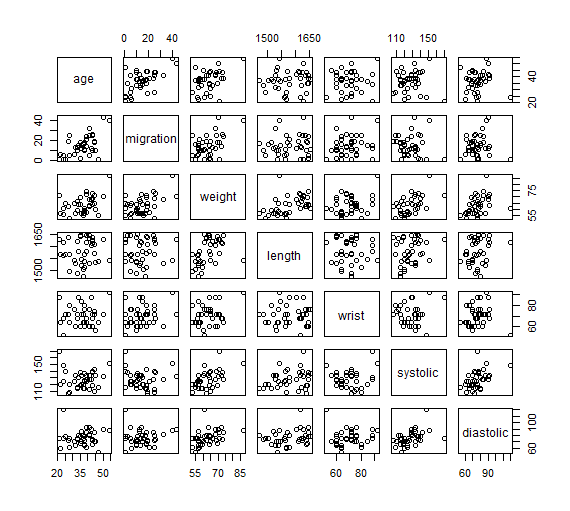
\includegraphics[scale=0.6]{../results/Pairs.png}
      \caption{Pairwise scatterplots of the dataset peruvians}
      \label{fig:Pairs}
    \end{figure}
    
    \subsection*{2}
    Using the Pearson (rank?) correlation test for all variables against migration we obtain the following results:
    \newline
    \begin{tabular}{|c|c|c|c|c|c|c|c|}
    \hline 
     & age & migration & weight & length & wrist & systolic & diastolic \\ 
    \hline 
    migration & 0.47605753 & 1 & 0.35069559 & 0.08458432 & 0.21934983 & -0.16842856 & 0.07514098 \\ 
    \hline 
    \end{tabular} 
    
    Age was the most obviously correlated variable between migration when the pairs scatter plots (Fig: \ref{fig:Pairs}), and age is the most correlated variable with migration.
    Weight is the second most correlated variable with migration, ...
    
    \section{Exercise 2}
    \subsection*{1}
    
    Two sample t-test assumes that both samples come from a normal population.
    Results of t-test are that we accept the null hypothesis that the means are the same, but as this test is not suitable for data that is not normally distributed this information doesnt actually tell us anything. The 95\% confidence interval is [-4.7405,559.5859] with mean of x = 441.9846 mean of y = 164.5619.
    The Mann-Whitney test: W=473, p-value = 0.01383
    Kolmogorov-Smirnov test: D = 0.4231, p-value = 0.01905
    
    \subsection*{2}
    t-test: t=2.4246, p-value = 0.01956, 95\% confidence interval [1.2021,13.0713], mean x=17.068, mean y= 9.9313
    Mann-Whitney test: The Mann-Whitney test: W=473, p-value = 0.01383
    Kolmogorov-Smirnov test: D = 0.4231, p-value = 0.01905
    
    \subsection*{3}
    t-test: t=2.5968, p-value=0.0124, 95\% [0.2196,1.7236], mean x = 3.8789, mean y = 2.9073
    Mann-Whitney test: The Mann-Whitney test: W=473, p-value = 0.01383
    Kolmogorov-Smirnov test: D = 0.4231, p-value = 0.01905
    
\end{document}